\documentclass[a4paper]{article}
\usepackage[utf8]{inputenc}
\usepackage[T1]{fontenc}
\usepackage{times}
\usepackage[margin=3cm]{geometry}

% German
%\usepackage[ngerman]{babel}
% English
\usepackage[english]{babel}

\usepackage[round,authoryear]{natbib}
\usepackage{amsmath,amssymb,amsthm}
\usepackage[hyphens]{url}
\usepackage{graphicx}
\usepackage{booktabs}

\usepackage{lipsum}

% German
%\newtheorem{definition}{Definition}
%\newtheorem{satz}{Satz}
% English
\newtheorem{definition}{Definition}
\newtheorem{theorem}{Theorem}

% TODO
\author{A. Student (\textit{remember to remove ID for the first draft and peer review!})}
\title{The title (\textit{which should really have more than two words, but should not be longer than two lines})}
\date{\today}

\begin{document}

\maketitle

\begin{abstract}
  \lipsum[1]
\end{abstract}

\section{Introduction}
\label{sec:intro}
This sentence is supported by a reference \citep{chaum1981untraceable}.
This sentence is justified with multiple references \citep{chaum1981untraceable,shamir1979how}.
\citet{alley2018craft} as well as \citet{strunk1999elements} use in-line references.

\lipsum[4]

\section{Background}
\label{sec:background}

\lipsum[1]
\begin{theorem}[Incompleteness theorem, \citeauthor{godel1931formal}, \citeyear{godel1931formal}]~\\
    If $c$ be a given recursive, consistent class of formulae, then the
    propositional formula which states that $c$ is consistent is not
    $c$-provable; in particular, the consistency of $P$ is unprovable in $P$, it
    being assumed that $P$ is consistent.
\end{theorem}

\subsection{First background topic}
\label{subsec:first-background}

\begin{figure}
    \centering
    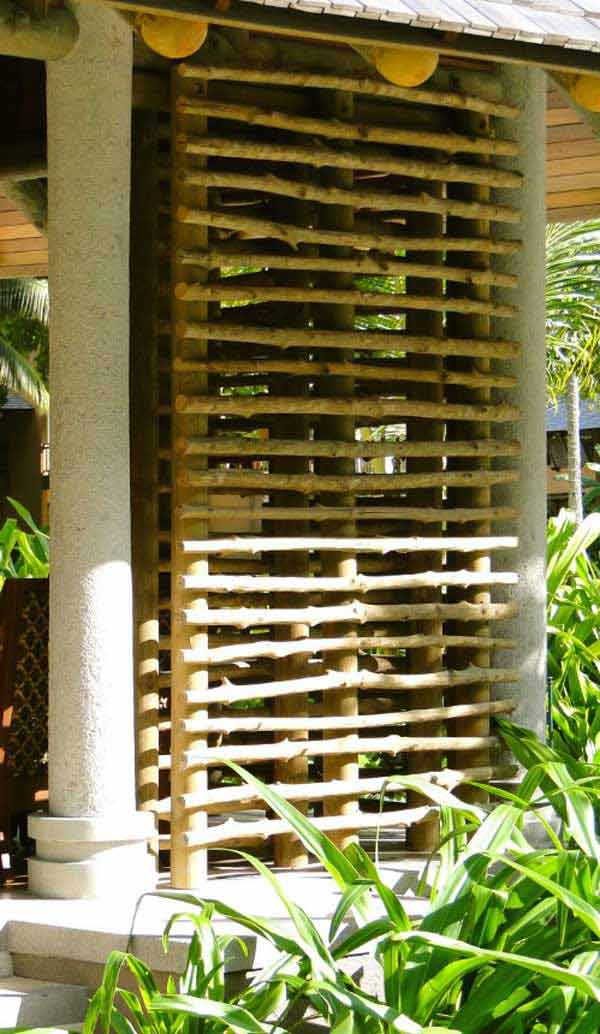
\includegraphics[width= 0.3\textwidth]{figures/privacy-screen}
    \caption{An example privacy mechanism}
    \label{fig-privacy-screen}
\end{figure}

\lipsum[3]
(See Figure~\ref{fig-privacy-screen}.)


\subsection{Second background topic}
\label{subsec:second-background}
\lipsum[2]
(See Table~\ref{tab:example}.)

\begin{table}
	\centering
	\begin{tabular}{p{3cm}ll}
		\toprule
		Header line & Column 2 & Column 3 \\
		\midrule
		Content line & 2 & 3 \\
		Another content line to showcase wrapping of table cells & 2 & 3 \\
		\bottomrule
	\end{tabular}
\caption{An example table}
\label{tab:example}
\end{table}

\section{Main content}
\label{sec:main}

Note that you \textit{must} rename this section to indicate \textit{what the content is}.


\section{Another topic in the main content}
\label{sec:anohter-topic}

Your ``main content'' can be split into as many sections as needed.


\section{Related work}
\label{sec:relwork}

Here, you include short descriptions of similar work and explain \textit{how} they are different from the main content you have presented.

Level of detail similar to an abstract. 

Note that you may include the related work as a subsection in the Background Section~\ref{sec:background}. 


\section{Conclusion}
\label{sec:conclusion}
\lipsum[3]

\section{Use of generative digital tools}

The use of AI tools must always be declared completely and transparently. 
For examples of how to do this, please see the DMI guidance: \url{https://dmi.unibas.ch/fileadmin/user_upload/dmi/Studium/Computer_Science/Diverses/Wegleitungen/Dokumente_2023/Guidance_on_AI_in_teaching_in_Computer_Science.pdf}.


\bibliographystyle{apalike}

\bibliography{references}


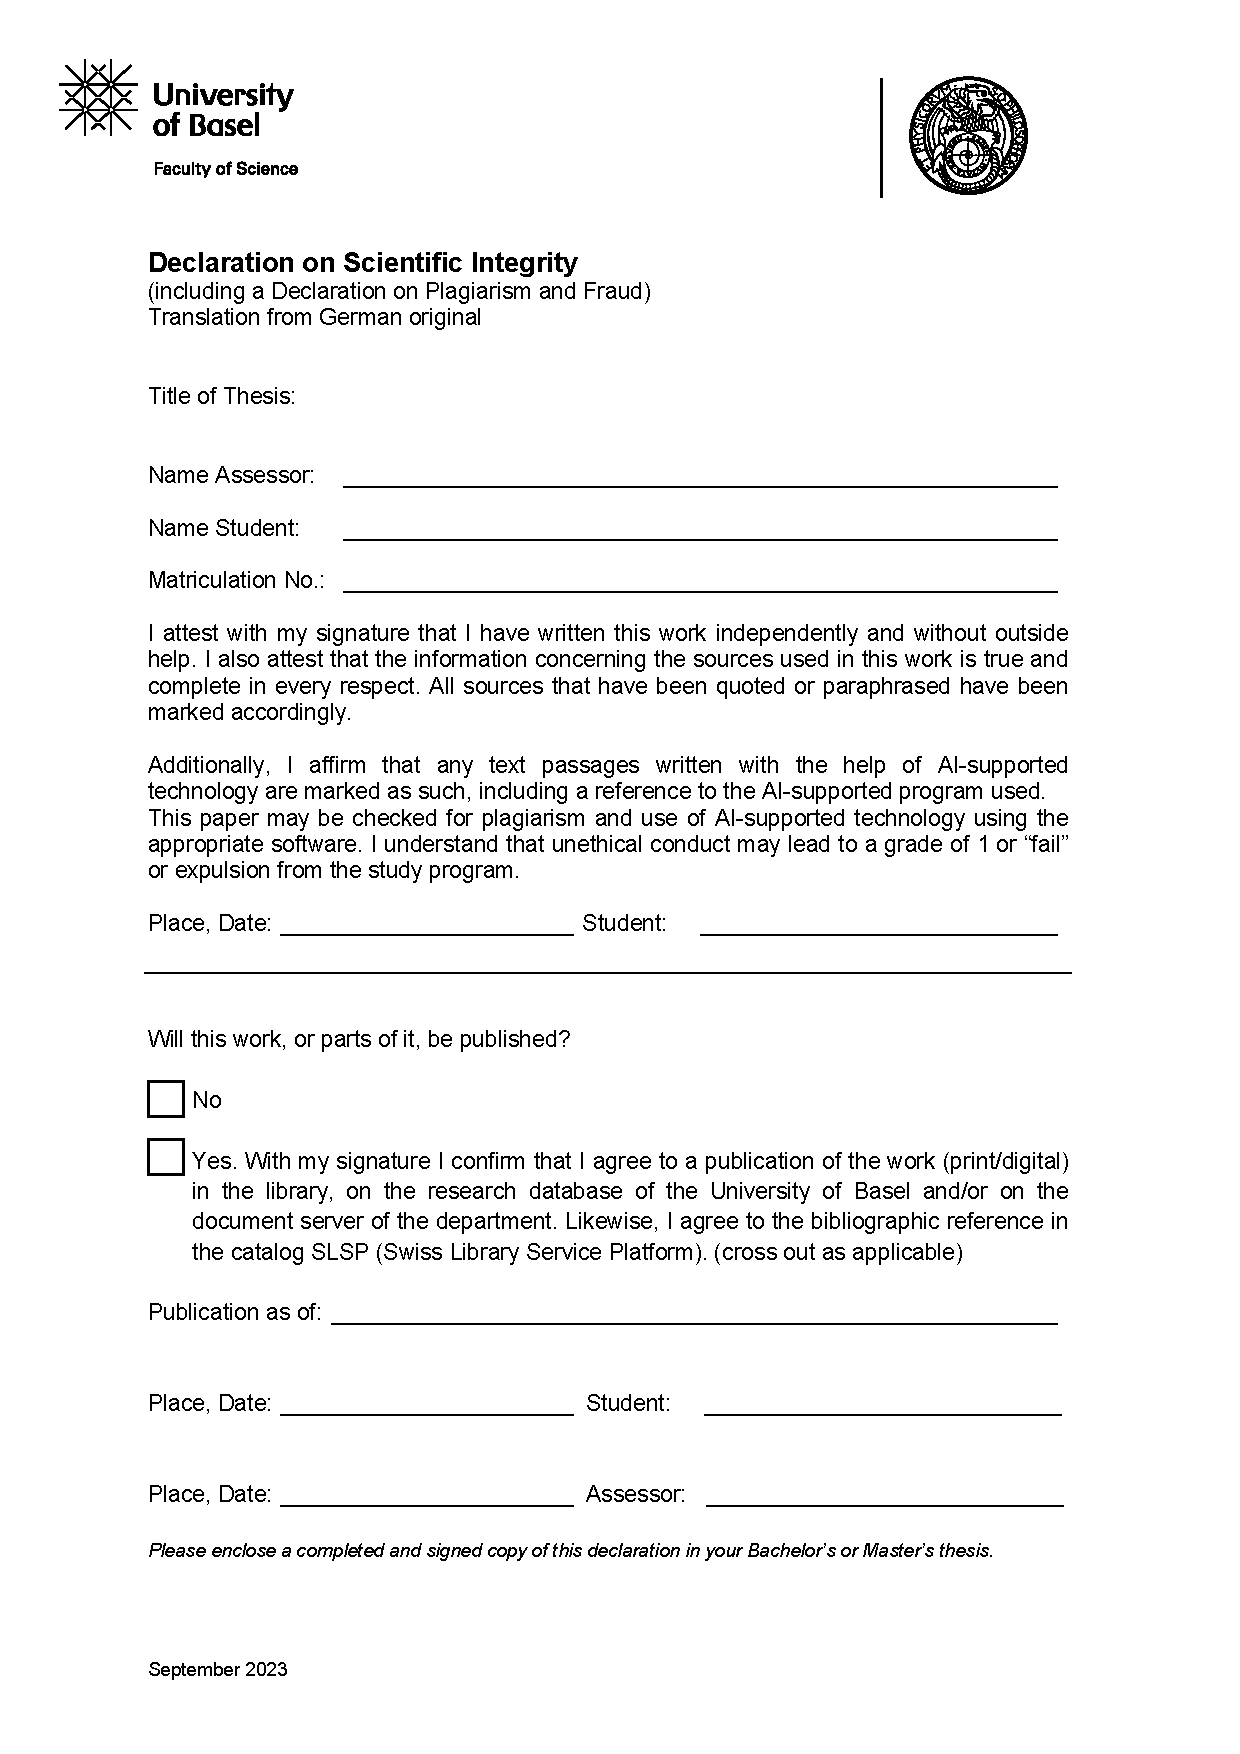
\includegraphics[width=\textwidth]{wissensch_Redlichkeit_E_09-2023}


\end{document}
